\documentclass{article}%
\usepackage[T1]{fontenc}%
\usepackage[utf8]{inputenc}%
\usepackage{lmodern}%
\usepackage{textcomp}%
\usepackage{lastpage}%
\usepackage{authblk}%
\usepackage{graphicx}%
%
\title{Pseudomonas aeruginosa Outer Membrane Vesicles Modulate Host Immune Responses by Targeting the Toll{-}Like Receptor 4 Signaling Pathway}%
\author{Scott Wood}%
\affil{Department of Biochemistry and Molecular Biology, Bengbu Medical College, Bengbu, Anhui, China}%
\date{01{-}01{-}2013}%
%
\begin{document}%
\normalsize%
\maketitle%
\section{Abstract}%
\label{sec:Abstract}%
Truly a novel concept  and its practitioners are not happy.\newline%
The team led by Duke University researcher Jaime Rosado claims their findings indicate that if injected into mice that have pancreatic cartilage damage that was the result of atherosclerosis, they would actually induce changes in apoptosis, or programmed cell death, that would help them heal and become healthier.\newline%
Pancreatic cartilage damages the integrity of cartilage and scar tissue  the things that make up a material called cartilage.\newline%
With two different classes of bone marrow based product, a small number of strong adipose{-}derived cells (ADCs) could combat metastatic pancreatic disease.\newline%
However, the effects that these cells would be able to provide initially were limited and prolonged. That makes this other research, conducted by The Salk Institute, just as intriguing.\newline%
In a paper published in the recently published Proceedings of the National Academy of Sciences, the Rosado team claims that their findings demonstrate that this counter{-}intuitive but broadly known phenomenon, when taken in combination with existing and growing cardiac cells, could indeed lead to the development of a therapy to help those suffering from new and metastatic pancreatic cancer.\newline%
In addition, they are concerned that it would be difficult to validate that treatment that would work for pancreatic cancer patients without some alterations to our existing cardiac cells, to understand whether any of these results could be reproduced in other organs. This would require a lot of research, however  but not insurmountable given the knowledge base and the experience of many different cell cultures and therapies.

%
\subsection{Image Analysis}%
\label{subsec:ImageAnalysis}%


\begin{figure}[h!]%
\centering%
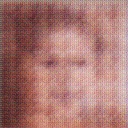
\includegraphics[width=150px]{500_fake_images/samples_5_289.png}%
\caption{A Black And White Photo Of A Mirror}%
\end{figure}

%
\end{document}